% Options for packages loaded elsewhere
\PassOptionsToPackage{unicode}{hyperref}
\PassOptionsToPackage{hyphens}{url}
%
\documentclass[
  ignorenonframetext,
]{beamer}
\usepackage{pgfpages}
\setbeamertemplate{caption}[numbered]
\setbeamertemplate{caption label separator}{: }
\setbeamercolor{caption name}{fg=normal text.fg}
\beamertemplatenavigationsymbolsempty
% Prevent slide breaks in the middle of a paragraph
\widowpenalties 1 10000
\raggedbottom
\setbeamertemplate{part page}{
  \centering
  \begin{beamercolorbox}[sep=16pt,center]{part title}
    \usebeamerfont{part title}\insertpart\par
  \end{beamercolorbox}
}
\setbeamertemplate{section page}{
  \centering
  \begin{beamercolorbox}[sep=12pt,center]{part title}
    \usebeamerfont{section title}\insertsection\par
  \end{beamercolorbox}
}
\setbeamertemplate{subsection page}{
  \centering
  \begin{beamercolorbox}[sep=8pt,center]{part title}
    \usebeamerfont{subsection title}\insertsubsection\par
  \end{beamercolorbox}
}
\AtBeginPart{
  \frame{\partpage}
}
\AtBeginSection{
  \ifbibliography
  \else
    \frame{\sectionpage}
  \fi
}
\AtBeginSubsection{
  \frame{\subsectionpage}
}
\usepackage{lmodern}
\usepackage{amsmath}
\usepackage{ifxetex,ifluatex}
\ifnum 0\ifxetex 1\fi\ifluatex 1\fi=0 % if pdftex
  \usepackage[T1]{fontenc}
  \usepackage[utf8]{inputenc}
  \usepackage{textcomp} % provide euro and other symbols
  \usepackage{amssymb}
\else % if luatex or xetex
  \usepackage{unicode-math}
  \defaultfontfeatures{Scale=MatchLowercase}
  \defaultfontfeatures[\rmfamily]{Ligatures=TeX,Scale=1}
\fi
% Use upquote if available, for straight quotes in verbatim environments
\IfFileExists{upquote.sty}{\usepackage{upquote}}{}
\IfFileExists{microtype.sty}{% use microtype if available
  \usepackage[]{microtype}
  \UseMicrotypeSet[protrusion]{basicmath} % disable protrusion for tt fonts
}{}
\makeatletter
\@ifundefined{KOMAClassName}{% if non-KOMA class
  \IfFileExists{parskip.sty}{%
    \usepackage{parskip}
  }{% else
    \setlength{\parindent}{0pt}
    \setlength{\parskip}{6pt plus 2pt minus 1pt}}
}{% if KOMA class
  \KOMAoptions{parskip=half}}
\makeatother
\usepackage{xcolor}
\IfFileExists{xurl.sty}{\usepackage{xurl}}{} % add URL line breaks if available
\IfFileExists{bookmark.sty}{\usepackage{bookmark}}{\usepackage{hyperref}}
\hypersetup{
  pdftitle={Transformation and transferral of acceptance following the 2019 Christchurch New Zealand Mosque Attacks},
  pdfauthor={Joseph Bulbulia, Psychology, Victoria University},
  hidelinks,
  pdfcreator={LaTeX via pandoc}}
\urlstyle{same} % disable monospaced font for URLs
\newif\ifbibliography
\usepackage{graphicx}
\makeatletter
\def\maxwidth{\ifdim\Gin@nat@width>\linewidth\linewidth\else\Gin@nat@width\fi}
\def\maxheight{\ifdim\Gin@nat@height>\textheight\textheight\else\Gin@nat@height\fi}
\makeatother
% Scale images if necessary, so that they will not overflow the page
% margins by default, and it is still possible to overwrite the defaults
% using explicit options in \includegraphics[width, height, ...]{}
\setkeys{Gin}{width=\maxwidth,height=\maxheight,keepaspectratio}
% Set default figure placement to htbp
\makeatletter
\def\fps@figure{htbp}
\makeatother
\setlength{\emergencystretch}{3em} % prevent overfull lines
\providecommand{\tightlist}{%
  \setlength{\itemsep}{0pt}\setlength{\parskip}{0pt}}
\setcounter{secnumdepth}{-\maxdimen} % remove section numbering
\ifluatex
  \usepackage{selnolig}  % disable illegal ligatures
\fi
\newlength{\cslhangindent}
\setlength{\cslhangindent}{1.5em}
\newlength{\csllabelwidth}
\setlength{\csllabelwidth}{3em}
\newenvironment{CSLReferences}[2] % #1 hanging-ident, #2 entry spacing
 {% don't indent paragraphs
  \setlength{\parindent}{0pt}
  % turn on hanging indent if param 1 is 1
  \ifodd #1 \everypar{\setlength{\hangindent}{\cslhangindent}}\ignorespaces\fi
  % set entry spacing
  \ifnum #2 > 0
  \setlength{\parskip}{#2\baselineskip}
  \fi
 }%
 {}
\usepackage{calc}
\newcommand{\CSLBlock}[1]{#1\hfill\break}
\newcommand{\CSLLeftMargin}[1]{\parbox[t]{\csllabelwidth}{#1}}
\newcommand{\CSLRightInline}[1]{\parbox[t]{\linewidth - \csllabelwidth}{#1}\break}
\newcommand{\CSLIndent}[1]{\hspace{\cslhangindent}#1}

\title{Transformation and transferral of acceptance following the 2019
Christchurch New Zealand Mosque Attacks}
\author{Joseph Bulbulia, Psychology, Victoria University}
\date{2021-JUNE-11}

\begin{document}
\frame{\titlepage}

\begin{frame}
\begin{block}{Muslim Acceptance Gap 2017/18\textbar{} Muslims 26.8\%
\textless{} 4 vs.~Immigrant 14\% \textless{} 4}
\protect\hypertarget{muslim-acceptance-gap-201718-muslims-26.8-4-vs.-immigrant-14-4}{}

\includegraphics{slides_files/figure-beamer/unnamed-chunk-1-1.pdf}
\end{block}

\begin{block}{Anti-Muslim prejudice is surprising}
\protect\hypertarget{anti-muslim-prejudice-is-surprising}{}
\begin{itemize}[<+->]
\item
  New Zealand's cultural diversity exceeds that of Australia, the United
  Kingdom, France, Germany, the Netherlands, and Scandinavia. Muslims
  are only a small part of this diversity (Shaver et al. 2017).
\item
  In 2018, New Zealand's Muslim, just over 1.5\% of the total
  population. The Islamic community has been present in New Zealand
  since at least 1874 (Shepard, 2006).
\item
  The New Zealand Muslim community is of diverse ethnic and cultural
  origins --- of those that affiliated with Islam in 2013, 26.9\% were
  born in Asia, 25.7\% in New Zealand, 23.3\% in the Middle East or
  Africa, and 21\% in the Pacific Islands (Center, 2013) (Shaver et al.
  2017). Thus, fewer than a quarter of New Zealand Muslims can be
  classified as `Arab.'
\item
  No record of any extremist Muslim group in New Zealand, nor have there
  been any reported attacks of Muslims on non-Muslims. Prejudice has no
  basis in experience.
\end{itemize}
\end{block}
\end{frame}

\begin{frame}{}
\protect\hypertarget{section}{}
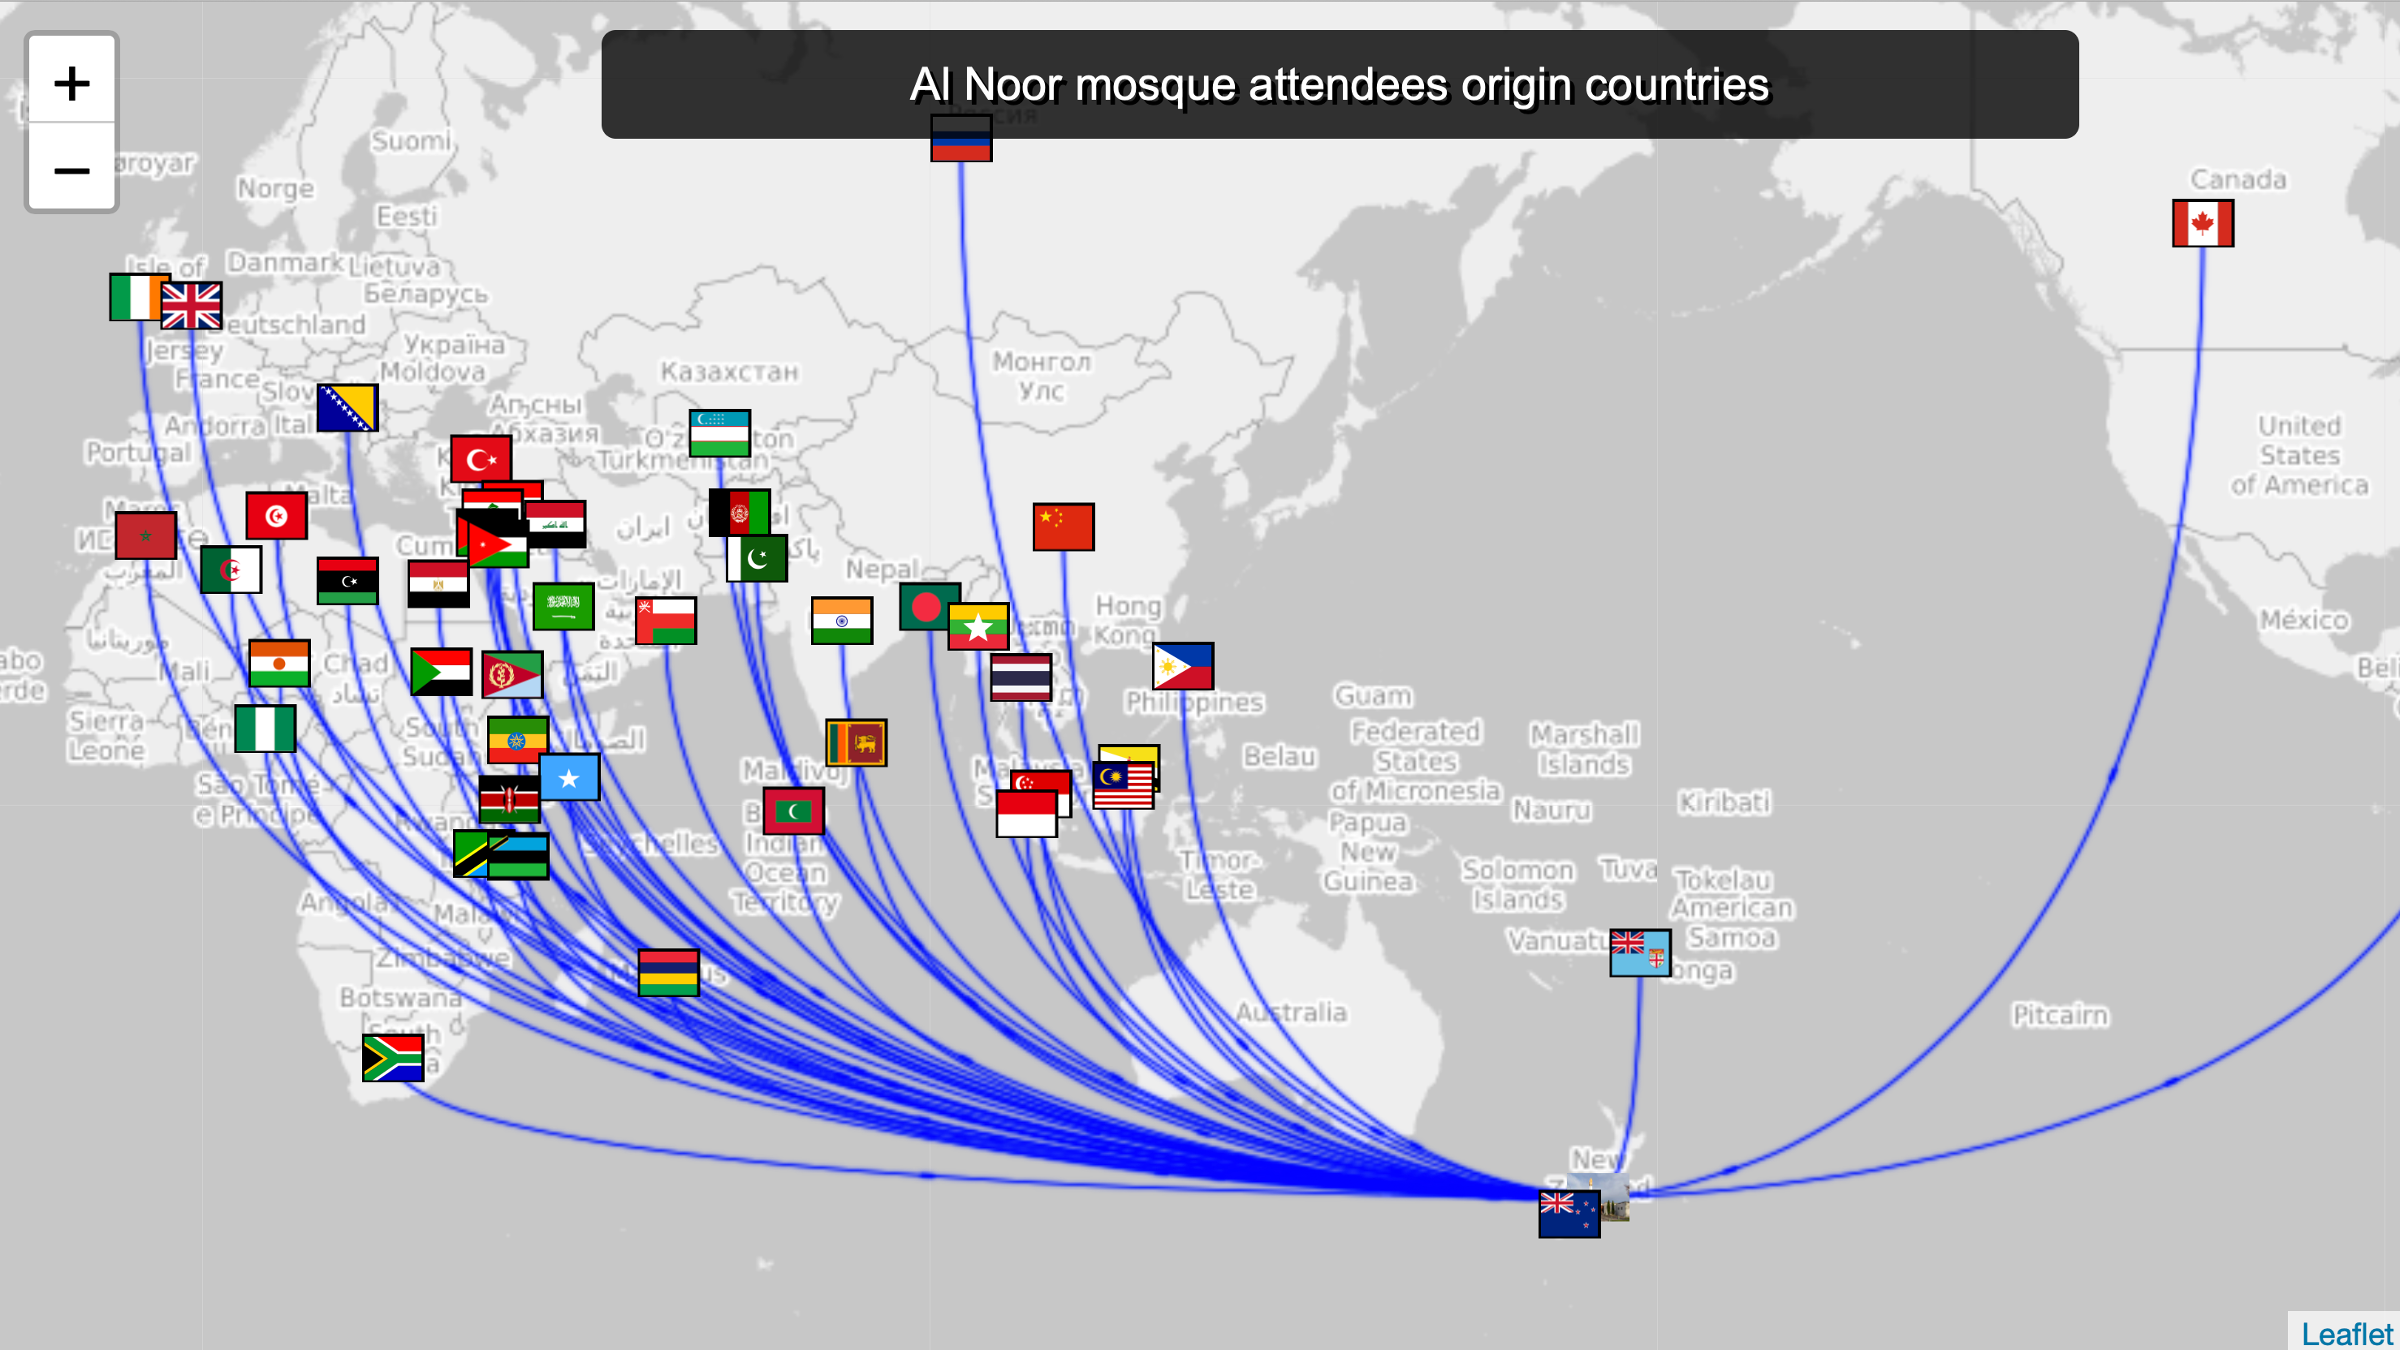
\includegraphics[width=33.33in]{alnoor}
\end{frame}

\begin{frame}{Why is there a Muslim Acceptance Gap?}
\protect\hypertarget{why-is-there-a-muslim-acceptance-gap}{}
\begin{block}{Muslims face a PR problem \textbar{} People know Muslims
from the news}
\protect\hypertarget{muslims-face-a-pr-problem-people-know-muslims-from-the-news}{}
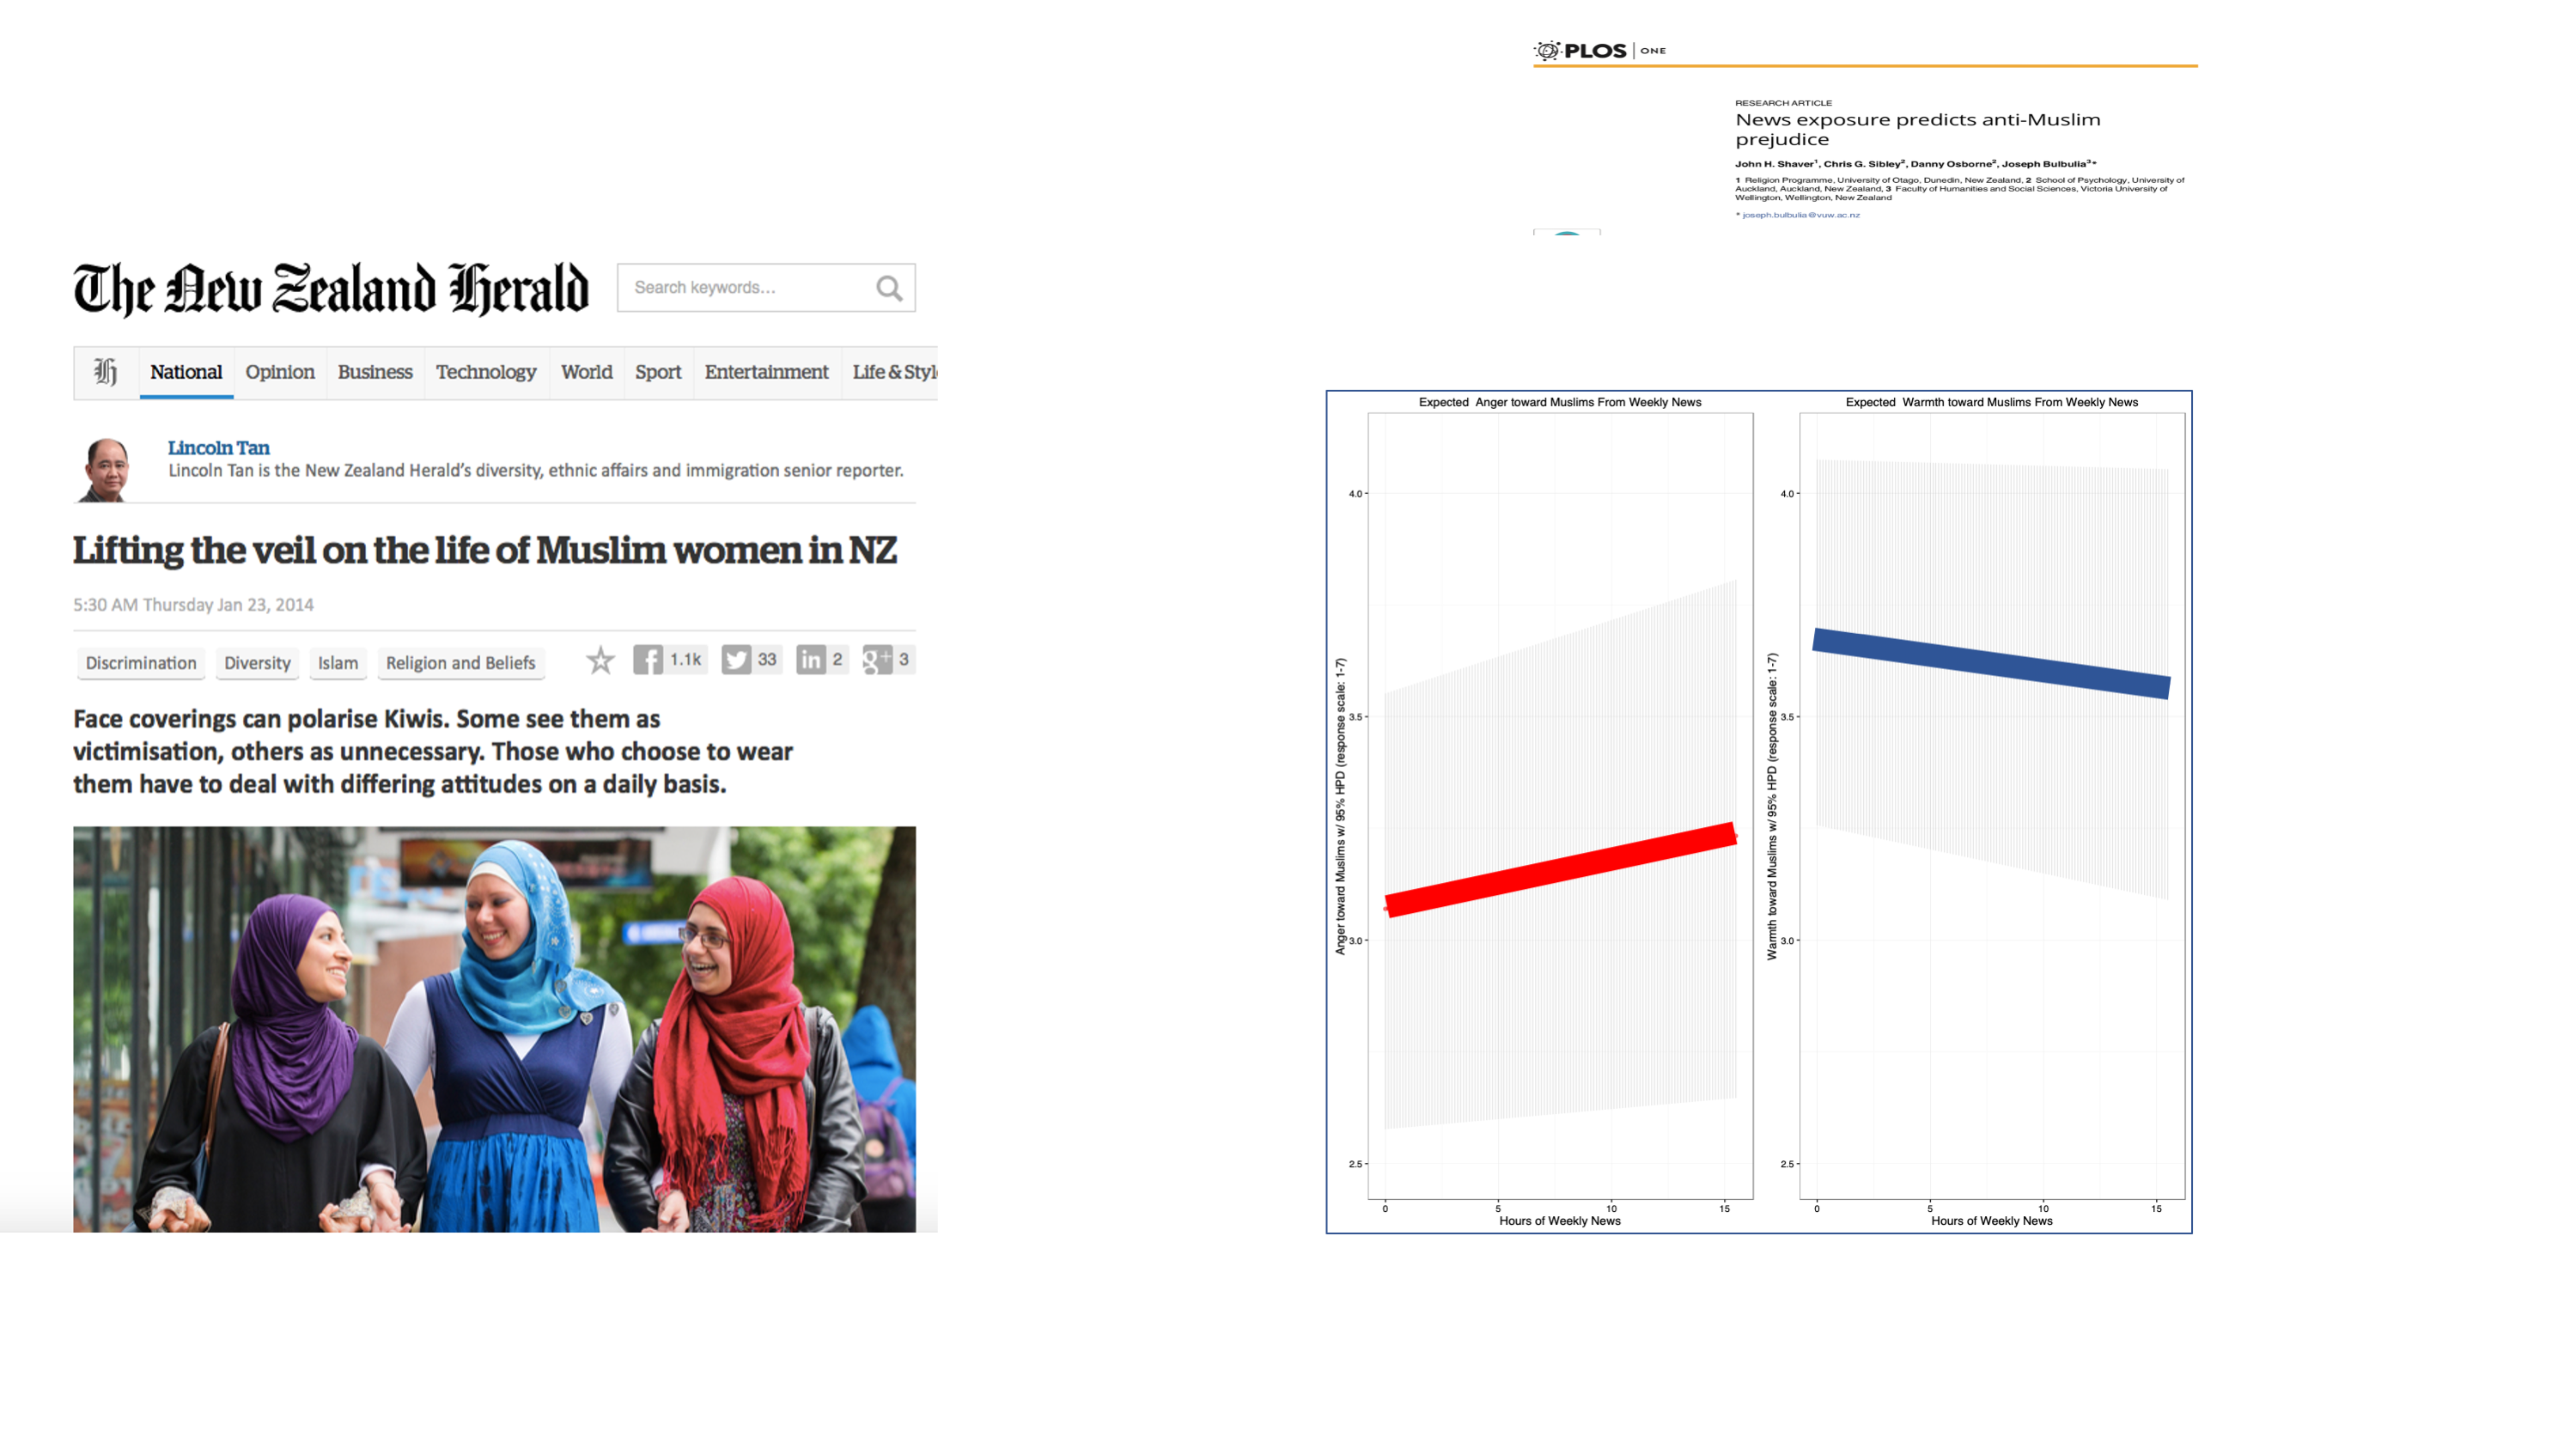
\includegraphics[width=41.65in]{pr}
\end{block}

\begin{block}{How did the 15 March 2019 Mosque attacks affect
prejudice?}
\protect\hypertarget{how-did-the-15-march-2019-mosque-attacks-affect-prejudice}{}
\includegraphics[width=41.65in]{shoot}
\end{block}

\begin{block}{}
\protect\hypertarget{section-1}{}
\includegraphics[width=41.65in]{shoot1}
\end{block}

\begin{block}{}
\protect\hypertarget{section-2}{}
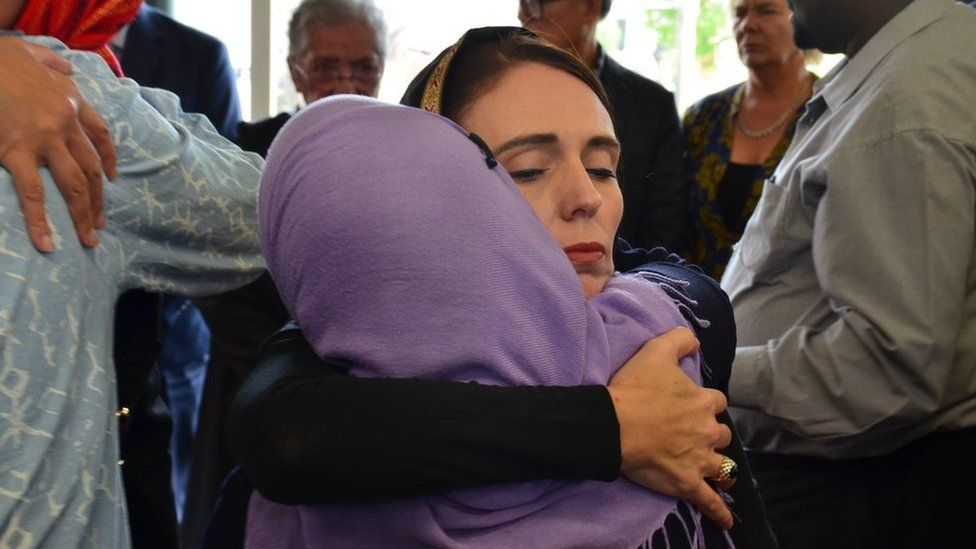
\includegraphics[width=13.56in]{jacinda2}

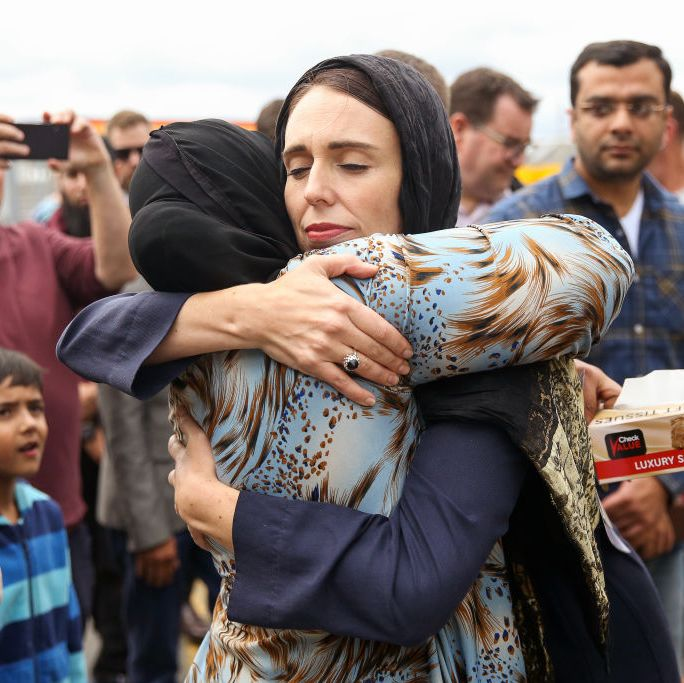
\includegraphics[width=9.5in]{jacinda}
\end{block}

\begin{block}{}
\protect\hypertarget{section-3}{}
\includegraphics[width=41.65in]{shoot2}
\end{block}

\begin{block}{}
\protect\hypertarget{section-4}{}
\includegraphics[width=41.65in]{shoot3}
\end{block}

\begin{block}{}
\protect\hypertarget{section-5}{}
\includegraphics[width=41.65in]{shoot4}
\end{block}

\begin{block}{}
\protect\hypertarget{section-6}{}
\includegraphics[width=41.65in]{al_noor_men}
\end{block}

\begin{block}{Muslim Acceptance Gap Post Shootings 2019/20 \textbar{}
Muslims 18.3\% \textless{} 4 (26.8\%) vs.~Immigrant 10.6\% \textless{} 4
(14\%)}
\protect\hypertarget{muslim-acceptance-gap-post-shootings-201920-muslims-18.3-4-26.8-vs.-immigrant-10.6-4-14}{}

\includegraphics{slides_files/figure-beamer/unnamed-chunk-12-1.pdf}

\includegraphics{slides_files/figure-beamer/unnamed-chunk-12-2.pdf}
\end{block}

\begin{block}{How did the 15 March 2019 Mosque attacks affect prejudice?
\textbar{} Here, we use Pre/Post Data from The New Zealand Attitudes and
Values Study}
\protect\hypertarget{how-did-the-15-march-2019-mosque-attacks-affect-prejudice-here-we-use-prepost-data-from-the-new-zealand-attitudes-and-values-study}{}
\begin{itemize}[<+->]
\item
  Planned 20-year longitudinal study, started by Prof.~Chris Sibley
  (Auckland), currently in its 12\(^{th}\) year.
\item
  Focus on personality, social attitudes, values, health, employment,
  religion, meaning-making, perfectionism, employment, experiences of
  discrimination, physical and psychological health, and environmental
  attitudes.
\item
  Postal questionnaire (retention \textasciitilde{} 80\%)
\item
  Sample frame drawn randomly from NZ Electoral Roll.
\item
  Large multidisciplinary research team (40 +)
\item
  Current sample contains \textasciitilde{} 38,000 unique people,
  \textgreater{} 1\% of the NZ adult population.
\item
  See:\href{https://www.psych.auckland.ac.nz/en/about/new-zealand-attitudes-and-values-study.html}{NZAVS}
\end{itemize}
\end{block}

\begin{block}{}
\protect\hypertarget{section-7}{}
\includegraphics[width=41.65in]{mail}
\end{block}

\begin{block}{}
\protect\hypertarget{section-8}{}

\includegraphics{slides_files/figure-beamer/timeline-1.pdf}
\end{block}

\begin{block}{}
\protect\hypertarget{section-9}{}
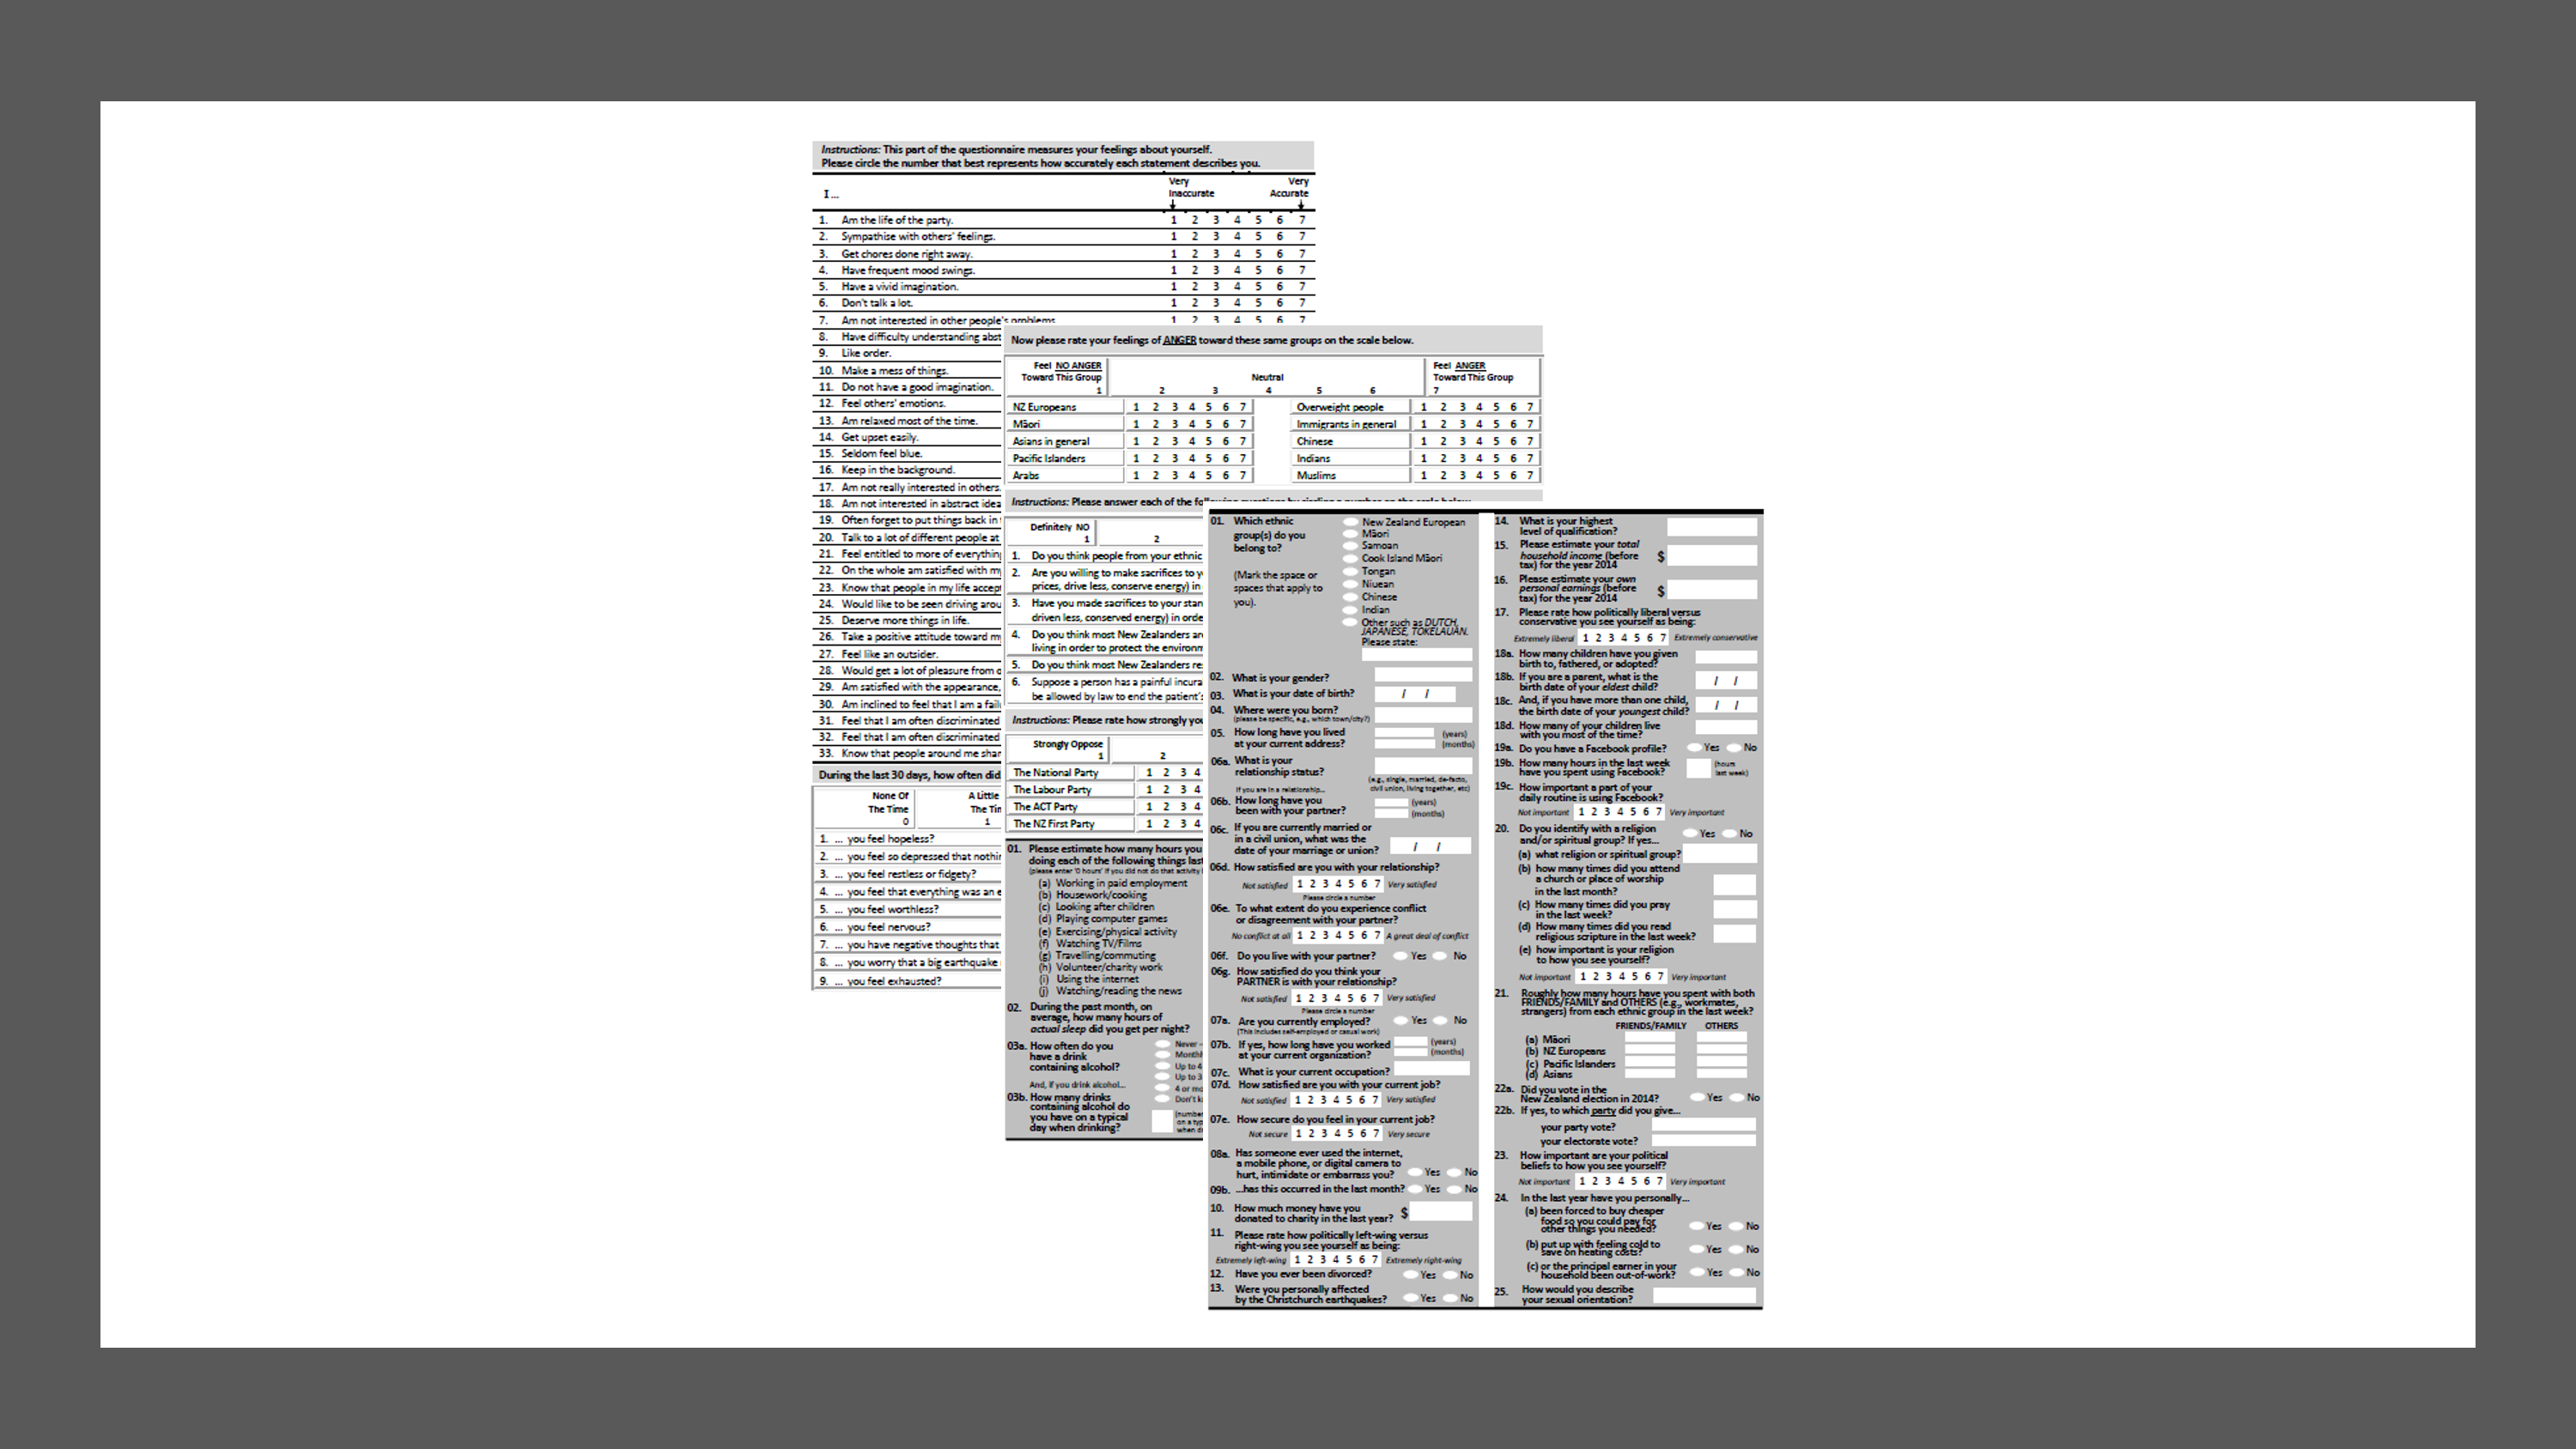
\includegraphics[width=41.67in]{questions}
\end{block}

\begin{block}{}
\protect\hypertarget{section-10}{}
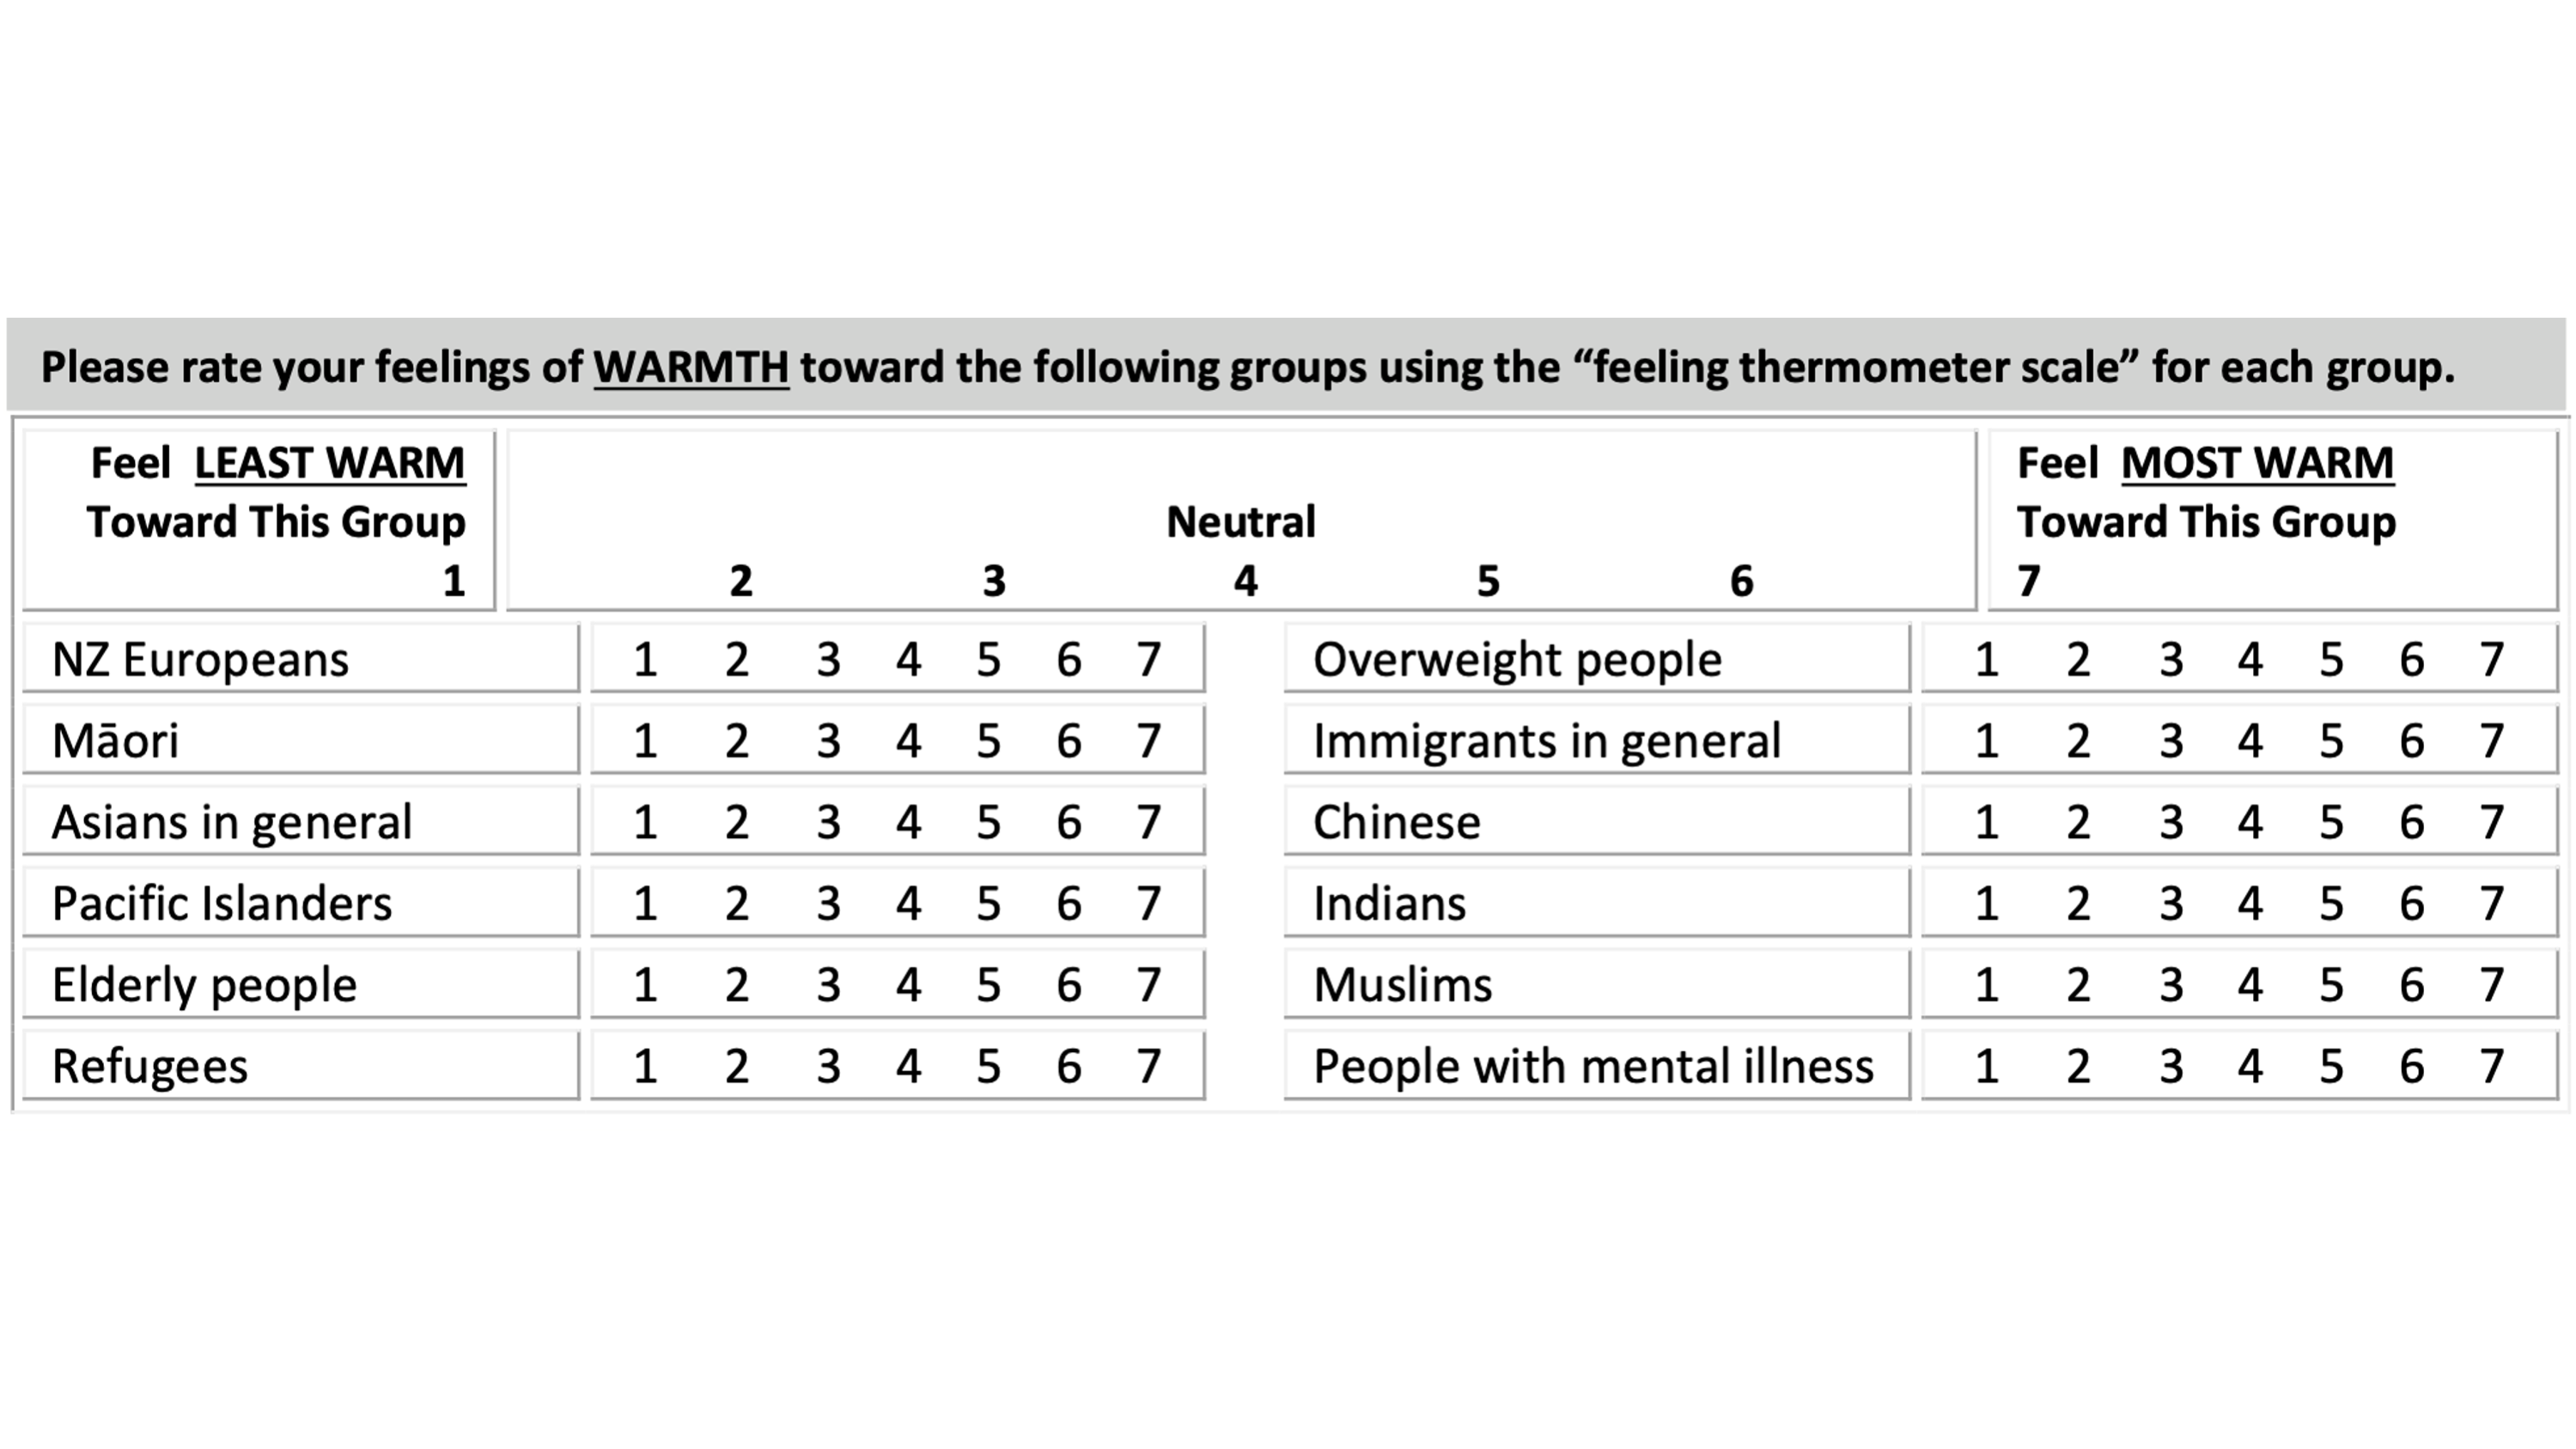
\includegraphics[width=41.65in]{scales}
\end{block}

\begin{block}{}
\protect\hypertarget{section-11}{}

\includegraphics{slides_files/figure-beamer/pptimeline-1.pdf}
\end{block}

\begin{block}{Numbers}
\protect\hypertarget{numbers}{}
\begin{table}

\caption{\label{tab:designtable}}
\centering
\begin{tabu} to \linewidth {>{\raggedright}X>{\raggedleft}X}
\hline
Pre\_PostATTACK & n\\
\hline
bsline\_w09 & 11481\\
\hline
pre\_w10 & 8120\\
\hline
pst\_w10 & 3361\\
\hline
pst\_w11 & 11481\\
\hline
\end{tabu}
\end{table}
\end{block}

\begin{block}{Model? \textbar{} Warmth to minority groups is slowly
increasing}
\protect\hypertarget{model-warmth-to-minority-groups-is-slowly-increasing}{}

\includegraphics{slides_files/figure-beamer/warmthtime2-1.pdf}
\end{block}

\begin{block}{}
\protect\hypertarget{section-12}{}

\includegraphics{slides_files/figure-beamer/unnamed-chunk-16-1.pdf}
\end{block}

\begin{block}{}
\protect\hypertarget{section-13}{}

\includegraphics{slides_files/figure-beamer/unnamed-chunk-17-1.pdf}
\end{block}

\begin{block}{}
\protect\hypertarget{section-14}{}

\includegraphics{slides_files/figure-beamer/unnamed-chunk-18-1.pdf}
\end{block}

\begin{block}{Results: Muslim-warmth boost}
\protect\hypertarget{results-muslim-warmth-boost}{}

\includegraphics{slides_files/figure-beamer/unnamed-chunk-19-1.pdf}
\end{block}

\begin{block}{Results: table}
\protect\hypertarget{results-table}{}
\captionsetup[table]{labelformat=empty,skip=1pt}
\begin{longtable}{lccccc}
\caption*{
\large Model Summary\\ 
\small \\ 
} \\ 
\toprule
Parameter & Coefficient & SE & 95\% CI & t(33692) & p \\ 
\midrule
\multicolumn{1}{l}{Fixed Effects } \\ 
\midrule
(Intercept) & 4.09 & 0.01 & (4.06, 4.11) & 302.11 & < .001 \\ 
Pre\_PostATTACK (pre\_w10) & 0.02 & 0.01 & (-7.41e-03, 0.04) & 1.39 & 0.165  \\ 
Pre\_PostATTACK (pst\_w10) & 0.31 & 0.02 & (0.28, 0.35) & 16.77 & < .001 \\ 
Pre\_PostATTACK (pst\_w11) & 0.26 & 0.01 & (0.24, 0.28) & 23.00 & < .001 \\ 
\midrule
\multicolumn{1}{l}{Random Effects } \\ 
\midrule
SD (Intercept: Id) & 1.16 &  &  &  &  \\ 
SD (Residual) & 0.92 &  &  &  &  \\ 
\bottomrule
\end{longtable}
\end{block}
\end{frame}

\begin{frame}{Were attitudes to non-normative outgroups affected?}
\protect\hypertarget{were-attitudes-to-non-normative-outgroups-affected}{}
\begin{block}{}
\protect\hypertarget{section-15}{}

\includegraphics{slides_files/figure-beamer/unnamed-chunk-21-1.pdf}
\end{block}

\begin{block}{}
\protect\hypertarget{section-16}{}

\includegraphics{slides_files/figure-beamer/unnamed-chunk-22-1.pdf}
\end{block}

\begin{block}{}
\protect\hypertarget{section-17}{}

\includegraphics{slides_files/figure-beamer/unnamed-chunk-23-1.pdf}
\end{block}

\begin{block}{}
\protect\hypertarget{section-18}{}

\includegraphics{slides_files/figure-beamer/unnamed-chunk-24-1.pdf}
\end{block}

\begin{block}{}
\protect\hypertarget{section-19}{}

\includegraphics{slides_files/figure-beamer/unnamed-chunk-25-1.pdf}
\end{block}
\end{frame}

\begin{frame}{Were attitudes to normative outgroups affected?}
\protect\hypertarget{were-attitudes-to-normative-outgroups-affected}{}
\begin{block}{}
\protect\hypertarget{section-20}{}

\includegraphics{slides_files/figure-beamer/unnamed-chunk-26-1.pdf}
\end{block}

\begin{block}{}
\protect\hypertarget{section-21}{}

\includegraphics{slides_files/figure-beamer/unnamed-chunk-27-1.pdf}
\end{block}

\begin{block}{}
\protect\hypertarget{section-22}{}

\includegraphics{slides_files/figure-beamer/unnamed-chunk-28-1.pdf}
\end{block}

\begin{block}{}
\protect\hypertarget{section-23}{}

\includegraphics{slides_files/figure-beamer/unnamed-chunk-29-1.pdf}
\end{block}

\begin{block}{}
\protect\hypertarget{section-24}{}

\includegraphics{slides_files/figure-beamer/unnamed-chunk-30-1.pdf}
\end{block}

\begin{block}{}
\protect\hypertarget{section-25}{}

\includegraphics{slides_files/figure-beamer/unnamed-chunk-31-1.pdf}
\end{block}

\begin{block}{Summary}
\protect\hypertarget{summary}{}

\includegraphics{slides_files/figure-beamer/unnamed-chunk-32-1.pdf}

\begin{itemize}[<+->]
\tightlist
\item
  Following the Christchurch Mosque attacks, warmth towards Muslim grew.
\item
  Despite this growth, warmth to Muslims still lags behind other groups.
\item
  There was shallower post-attack boost in warmth for non-mormative
  minorities.
\item
  The attacks did not affect warmth towards normative minorities.
\item
  It is unclear whether the boost to warm towards Muslims will be
  sustained.
\end{itemize}
\end{block}

\begin{block}{Importance of findings}
\protect\hypertarget{importance-of-findings}{}
\begin{itemize}[<+->]
\tightlist
\item
  Although the purpose of the Mosque attacks was to incite division, the
  attacks caused a strong boost in acceptance.
\item
  Within the next century, Muslims will become the global religious
  majority. Non-Muslims should better understand Muslim diversity.
\item
  New Zealanders value democratic freedom and fairness. It should be OK
  for people to believe or disbelieve after their conscience
\end{itemize}
\end{block}

\begin{block}{Thanks}
\protect\hypertarget{thanks}{}
\begin{itemize}[<+->]
\tightlist
\item
  Prof Chris G. Sibley \& the NZAVS team
\item
  NZAVS participants
\end{itemize}
\end{block}
\end{frame}

\begin{frame}{}
\protect\hypertarget{section-26}{}
\includegraphics[width=41.65in]{team}
\end{frame}

\begin{frame}{}
\protect\hypertarget{section-27}{}

\includegraphics[width=20.72in]{trt}

\begin{block}{Slides here}
\protect\hypertarget{slides-here}{}
\url{https://go-bayes.github.io/reports/posts/mus/}
\end{block}
\end{frame}

\begin{frame}{Extra slides}
\protect\hypertarget{extra-slides}{}
\begin{block}{}
\protect\hypertarget{section-28}{}
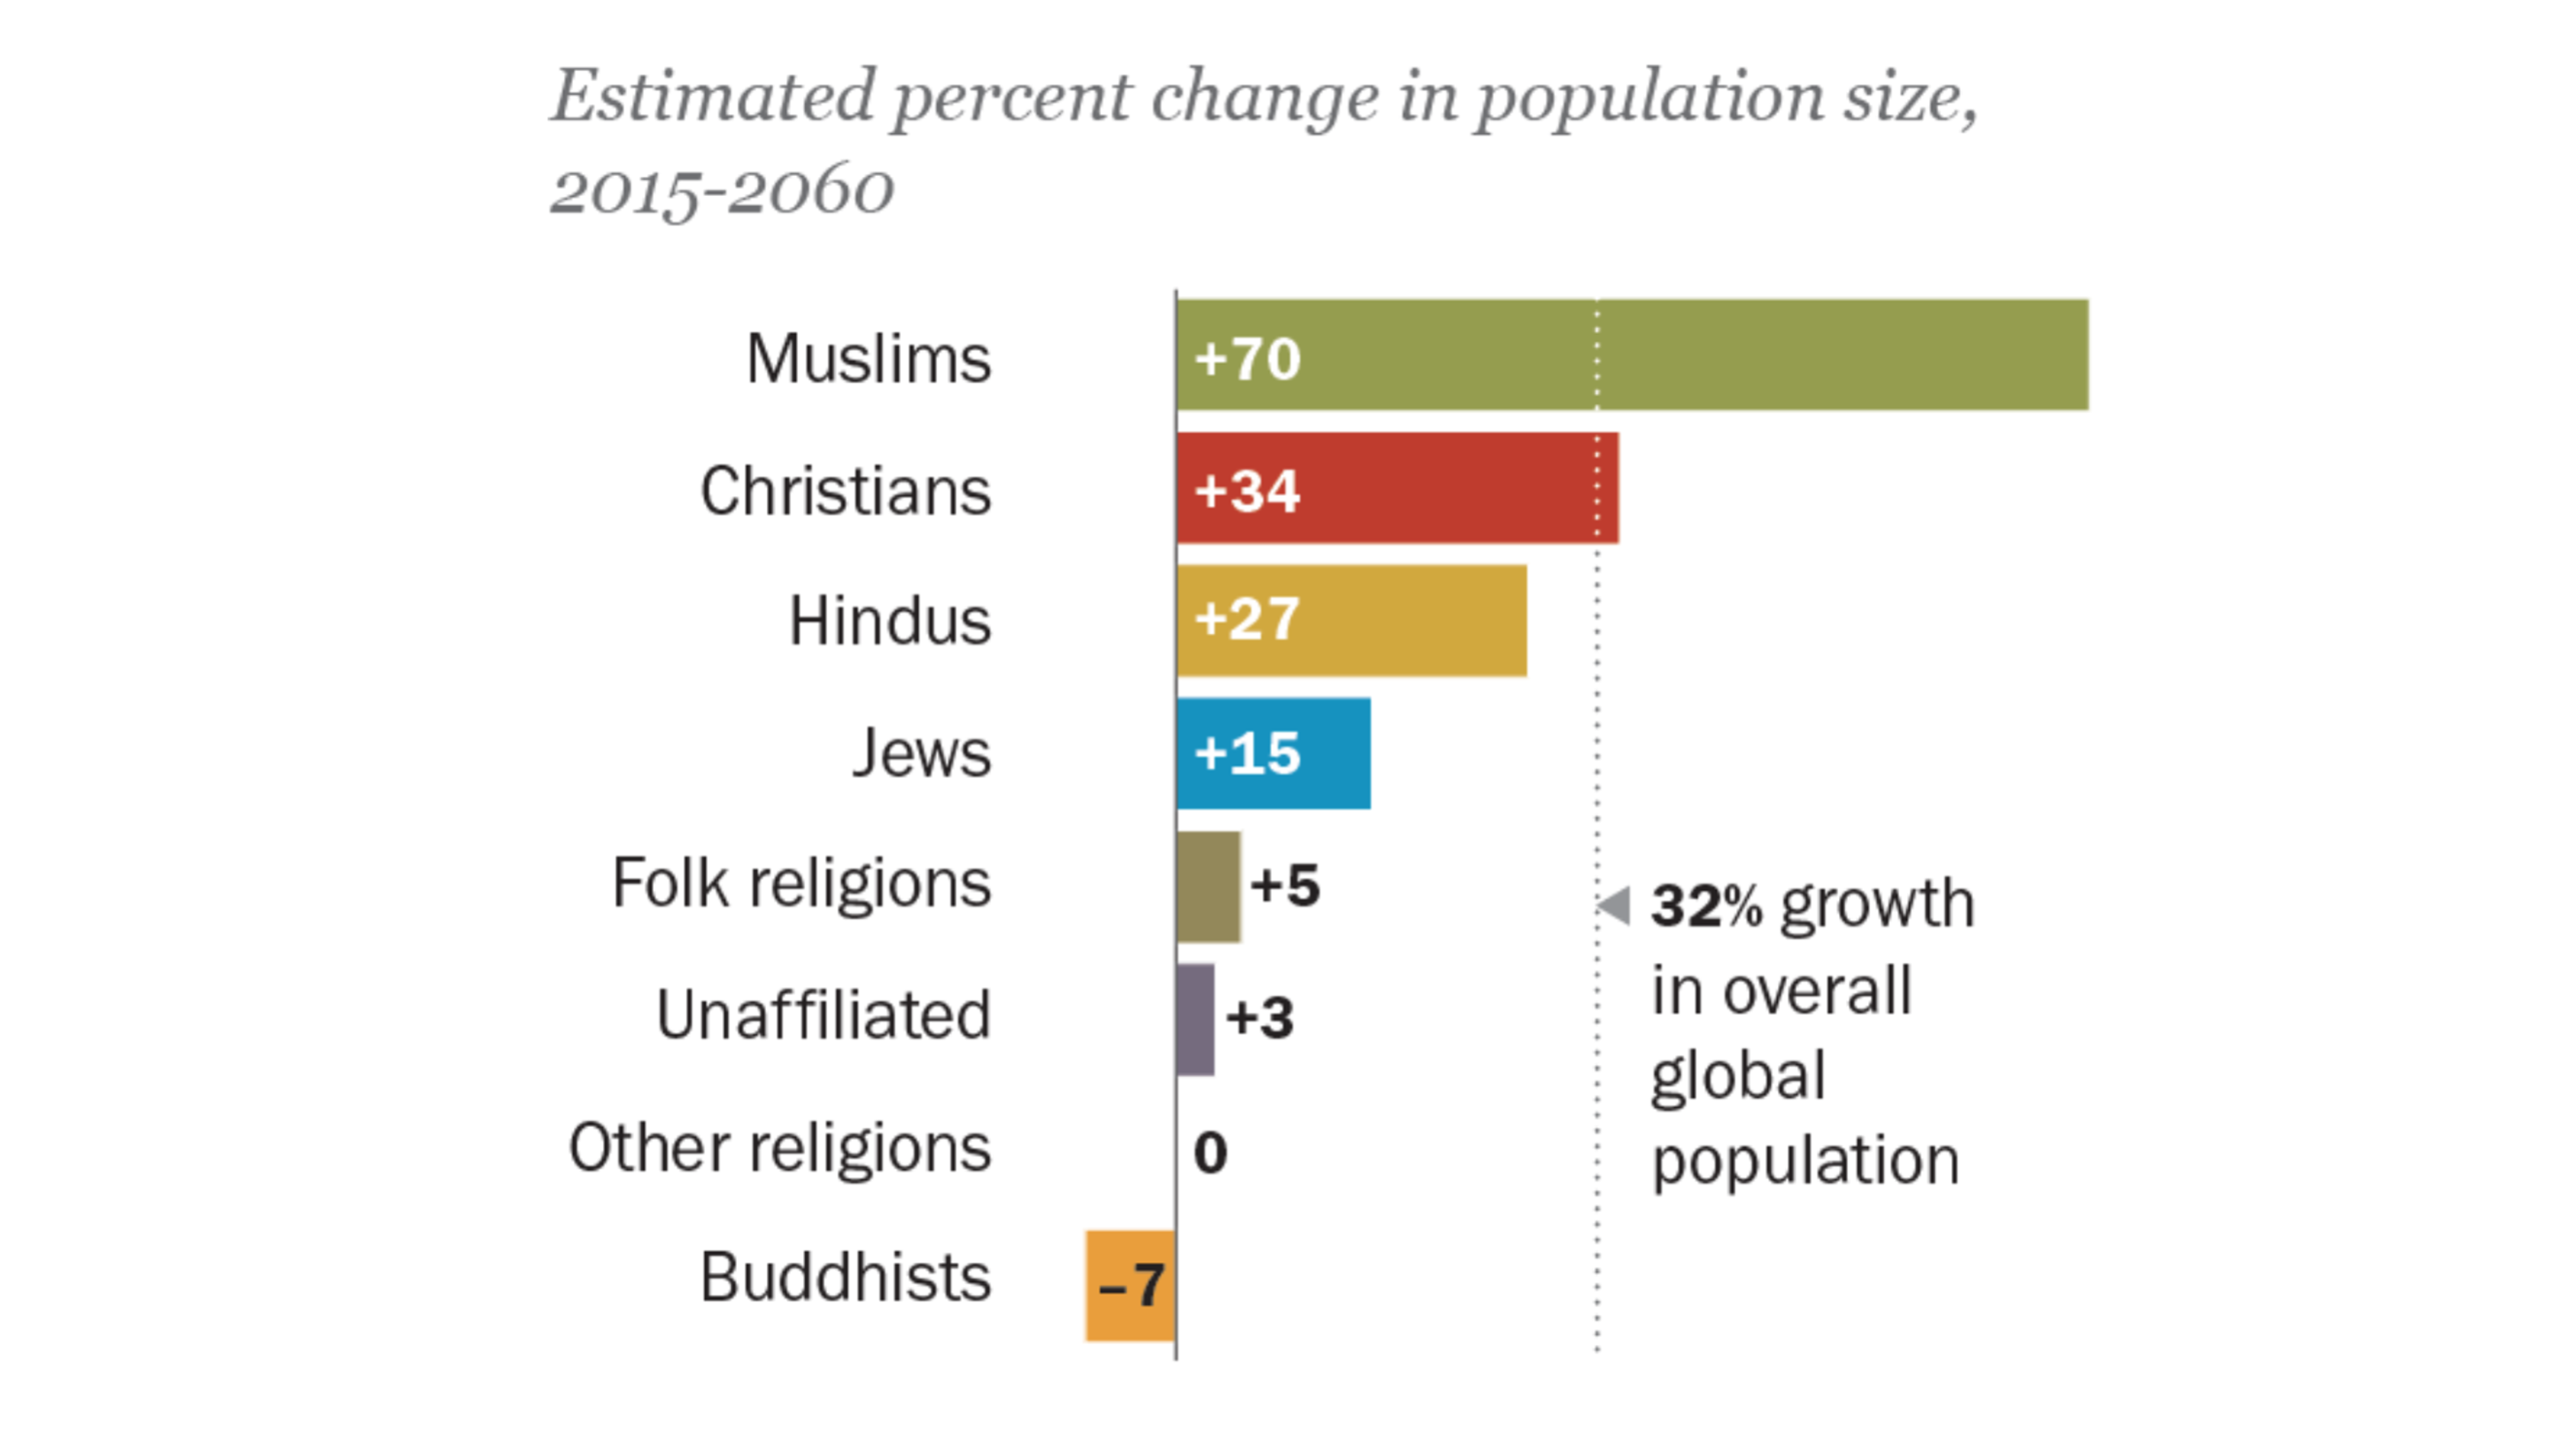
\includegraphics[width=41.65in]{grow1}
\end{block}

\begin{block}{}
\protect\hypertarget{section-29}{}
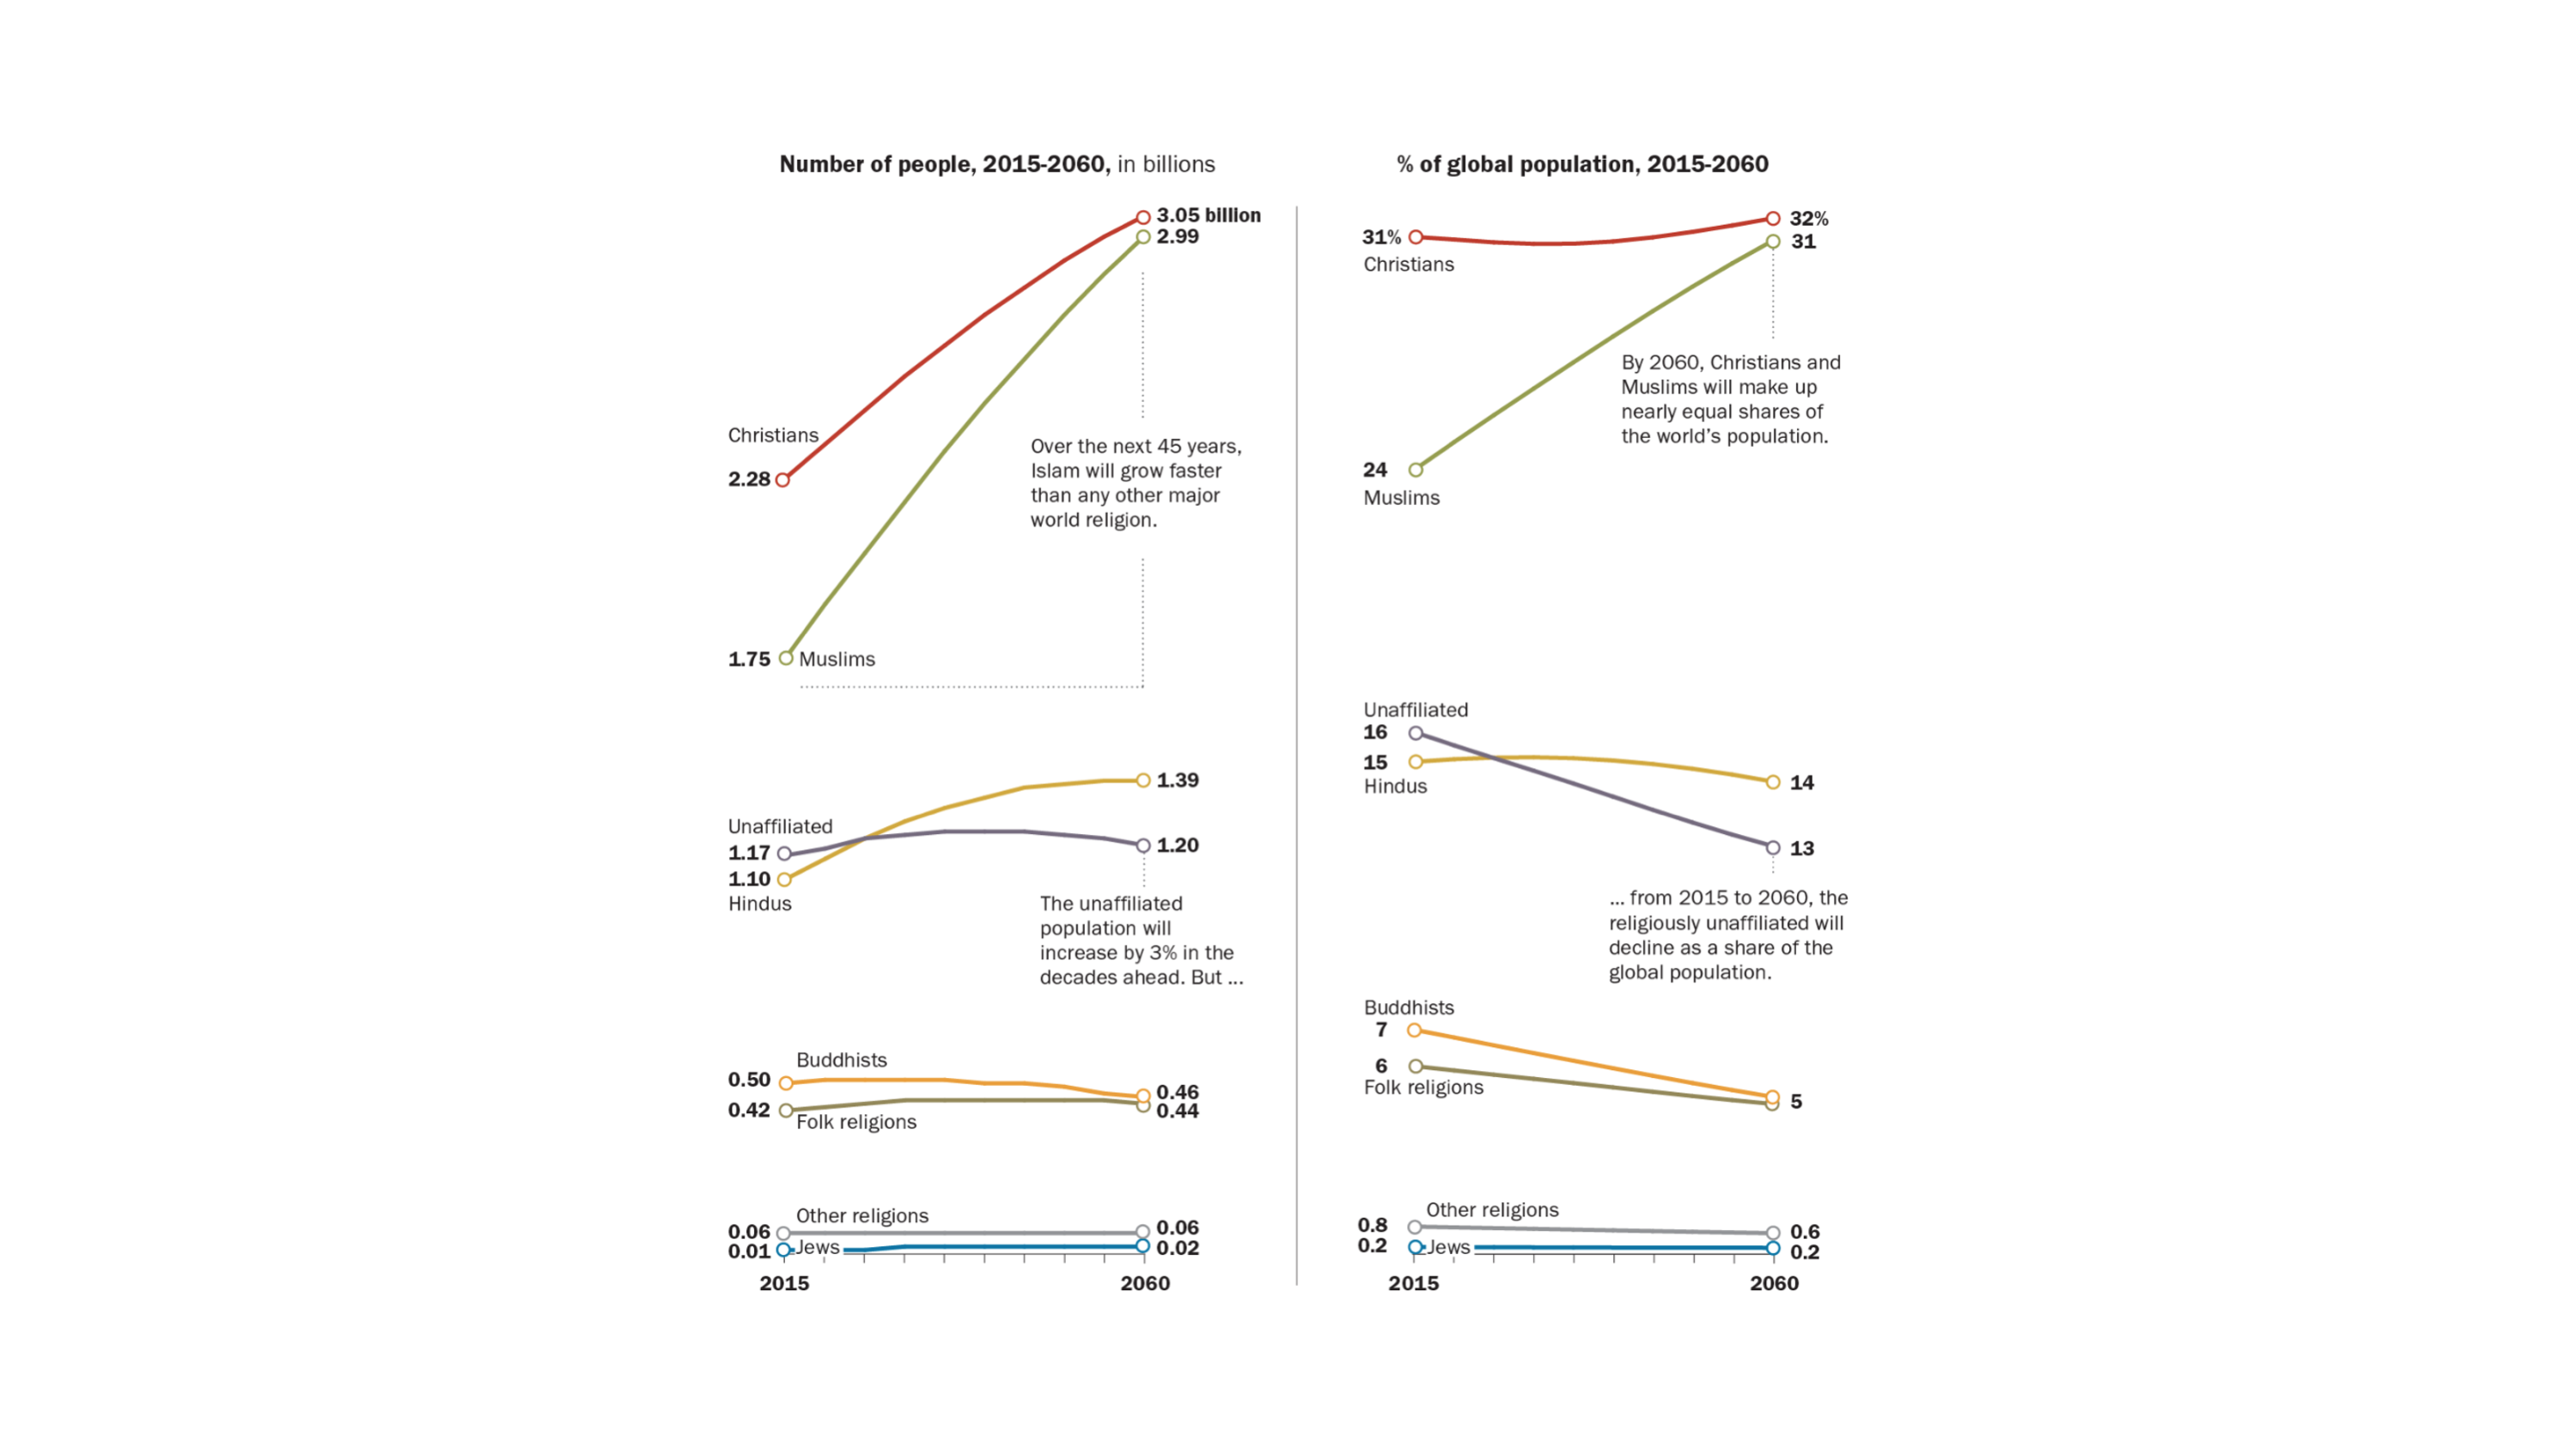
\includegraphics[width=41.65in]{grow2}
\end{block}

\begin{block}{Political conservatives also grew more accepting of
Muslims}
\protect\hypertarget{political-conservatives-also-grew-more-accepting-of-muslims}{}

\includegraphics{slides_files/figure-beamer/graphsmodelsPol-1.pdf}
\end{block}

\begin{block}{Bibliography}
\protect\hypertarget{bibliography}{}
\hypertarget{refs}{}
\begin{CSLReferences}{1}{0}
\leavevmode\hypertarget{ref-shaver2017news}{}%
Shaver, John H, Chris G Sibley, Danny Osborne, and Joseph Bulbulia.
2017. {``News Exposure Predicts Anti-Muslim Prejudice.''} \emph{PloS
One} 12 (3): e0174606.

\end{CSLReferences}
\end{block}
\end{frame}

\end{document}
